\section{Introduction}\pagenumbering{arabic}
The aim of this work is to develop and implement trajectory planning and motion control algorithms that allow a nano quadcopter to perform complex maneuvers at high speed. The backflip maneuver has been chosen as an example, because it is a challenging task even for an expert human driver, and it emphasizes the complex nonlinear behaviour of the drone. The complexity and speed of the maneuver is characterized by the fact that it takes less than a second to complete, during which the vehicle is able to make a full turn around one of the horizontal axes.

The maneuver is performed by miniature quadcopters, more generally micro aerial vehicles (MAVs). MAVs are a type of unmanned aerial vehicles (UAVs) that has small size and are usually autonomous. These vehicles are often designed based on bio-inspirations, i.e. they mimic the behaviour and flight capabilities of flying insects or birds. Due to the small-sized and low-power sensor and computer units, they are now continuously developed and applied both in industry and research. Their most common applications include military purposes (exploration and observation), search and rescue missions, aerial photography, distributed sensing and information processing while working in team, or agile maneuvering in a cluttered environment. Three micro aerial vehicles are shown in Figure \ref{fig:intro}: the first two developed for military applications, and the third for research and education.

Many common tasks of a miniature quadcopter, such as navigating in a cluttered environment or flying in strong wind require to perform complex, fast maneuvers that push the drones to their physical limits. In these cases, classical flight controllers designed for a linearized dynamical model are no longer applicable and more advanced control methods that exploit the entire operating domain are needed. These algorithms can be developed based on nonlinear control techniques, or machine learning approaches.

\begin{figure}[b]
    \centering
    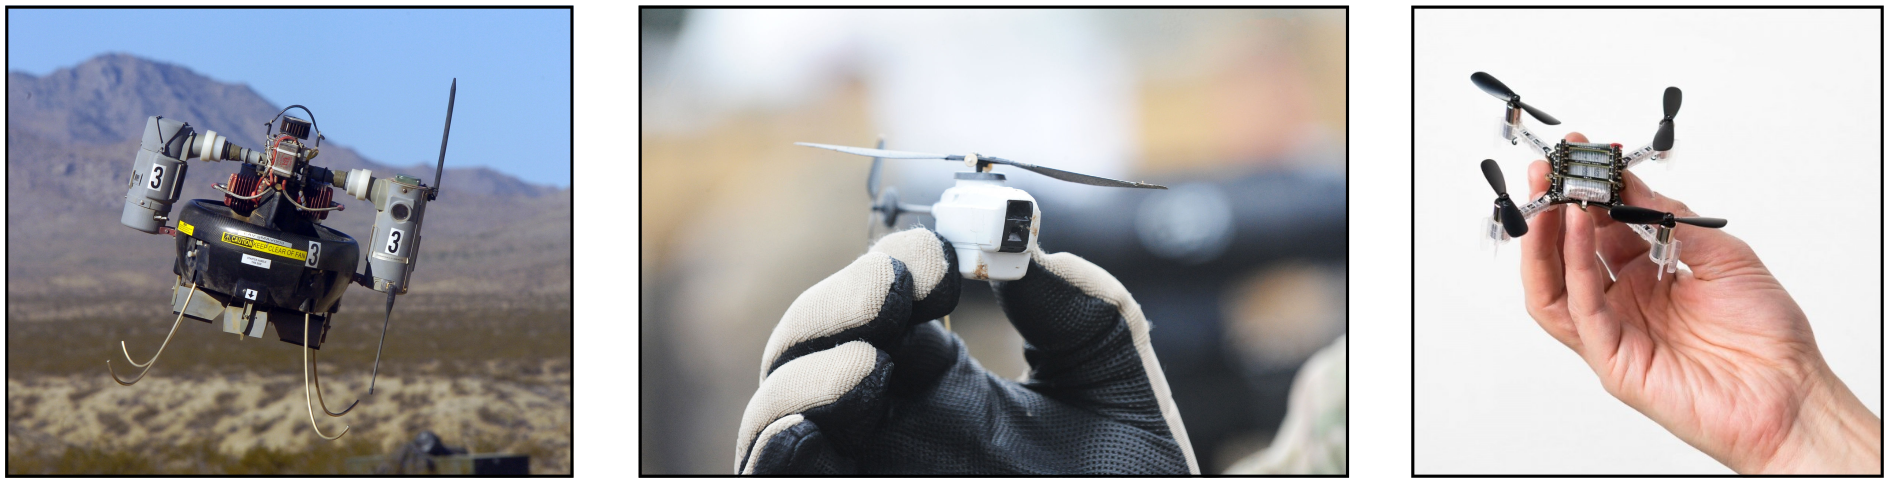
\includegraphics{Fig/intro.png}
    \caption{Micro aerial vehicles: RQ-16 T-Hawk (left), Black Hornet Nano (center), and Bitcrcaze Crazyflie 2.1 (right).}
    \label{fig:intro}
\end{figure}

At AIMotion Lab of ELKH SZTAKI there is a flying arena with five Bitcraze Crazyflie 2.1 miniature quadrotors. These drones are designed for research and education purposes, therefore they are both open hardware and open source, making it possible to implement our own algorithms on-board. Due to their low weight and relatively small mechanical power no on-board cameras can be used, therefore an external OptiTrack motion capture system provides position and orientation information for the drone, the data of which is fed back to the on-board controller via radio communication. With the highly reliable and precise localization, the Crazyflie is able to track complex trajectories with high performance using a suitable flight controller.

Backflipping with a quadcopter is an interesting control problem not only because it emphasizes the nonlinearity of the dynamical model, but also requires special considerations regarding the attitude representation and control. In the literature, there are several different approaches to perform the flip maneuver. In \cite{energy-quaternion}, energy-based control is applied to overcome the uncontrollability of the quadcopter at singular configurations to follow a circular or clothoidal reference trajectory. Machine learning approaches are utilized in many cases, for example to imitate the maneuver performed by an expert drone pilot with apprenticeship learning \cite{abbeel2010}, or design time-optimal trajectories with deep reinforcement learning \cite{drone-racing-deep-rl} and learn acrobatic maneuvers \cite{deep_acrobatics, quadrotor-control-rl}. 

A simple learning strategy for adaptive open-loop control is proposed in \cite{LSICRA2010}, based on the optimization of a parametric motion primitive sequence. As backflipping pushes the actuators of the quadcopter to their physical limits, the application of near-maximal and minimal control inputs are required. This approach builds on the theory of bang-bang control and first-principles motion primitive design to perform and optimize the flip maneuver. 

Geometric control is a nonlinear approach for attitude feedback control of rigid bodies in 3D space. In \cite{lelemc2010}, it is theoretically proven that geometric control is able to stabilize the orientation of a quadcopter in the whole operating domain based on differential geometric considerations and Lyapunov stability. A control law is proposed, on which other researchers build and extend for real-time trajectory generation and aggressive, agile maneuvering \cite{turpinkumar2011, mellinger2011} .

% have a wide range of industrial applications. Most common are search and rescue missions in disaster areas, or agricultural monitoring. It is also a popular topic in the field of systems and control engineering, because of the simplicity of a baseline dynamical model and mechanical design. However, the precise execution of aggressive, fast maneuvers requires advanced modelling and control techniques, which include the use of nonlinear or learning algorithms.


In this work, firstly the theoretical background of quadrotor dynamics and control is demonstrated. In Sections 3-4, two control approaches are proposed to perform a flip maneuver:  open-loop control based on motion primitive optimization, and geometric tracking control for an optimized reference trajectory. In Section 5, the simulation framework, implementation and results are discussed for the dynamical model of the Crazyflie 2.1 quadcopter. The experimental setup, implementation on the real robot, and  measurement results are demonstrated in Section 6, with a comparison of the two control approaches. Finally, the conclusion and future work are summarized in Section 7.
